%!TEX root = ../Technical_paper.tex
\section{System Evaluation}
\subsection{Camera hardware and control}
The image  processing of the camera frames on the raspberry can be a significant bottleneck for the system. With the current system setup running at 30fps, this means that the image processing time, containing frame readout and downstream processing of the images, has to be done in about $1/30s$ or 33 ms to achieve "real time" processing. The cameras use a rolling shutter instead of a global shutter. Since these cameras are designed to be of easy use for the normal consumer, they lack means of external synchronization. Attempting the synchronization of the data via Software further down the processing pipeline is therefore more reasonable.
\\To synchronize the reading start point of both cameras the system boots up to the point where all needed components are initialized. At this point the program waits for a start message from the parent system via UDP. The parent system send the start message at the end of its initialization phase via a UDP broadcast, ensuing that both Raspberry's get the message at the same time.\\
All automatic modes are turned of in the camera initialization phase and fixed values are loaded from a JSON file. To get the values for the JSON file a calibration step was implemented into the command line tool. The user-set calibration values can be written into a new JSON file and are directly loaded into the program after calibration is finished. Control over these parameters is crucial for achieving a constant color separation. The threshold values values for the color tracking also need to be initially calibrated. These values are dependent on the lighting situation and any change results in the need for re-calibration. To simplify this calibration a calibration function in the same fashion as the camera calibration was implemented.
\section{Image processing performance}
Initial investigation into code timings showed, that a bottleneck was the image optimization feature which applied an erosion an dilation to remove high frequency noise in the image. This operation brought the time up to 100 ms processing time when processing the whole frame area, making the algorithm  not usable for "real time" application.Removing this feature for whole image scans brought a major speed up in processing time. 
A test with lower resolution than 640x480 showed that the calculation time can be reduced furthermore. This confirmed that the ROI idea would be feasible for further performance optimization. A test at a frame resolution of 320x240 pixels reduced the processing time for all five colors to below 10 ms.\\
Performance measurement for tracking consistency with stationary color trackers was performed for a time period of 10.000 frames to get qualitative results. The sequential implementation showed an average processing time of 46 ms with a standard deviation of ~11 ms.\\
The same measurement were done with a finer time tracking on the single parts of the processing pipeline to get a finer timing resolution. 96\% of the processing time is taken up by the image stereo rectification (31 ms) and the color tracking(15 ms ).\\
Stereo rectification is usually done to ensure that the two used images have an aligned horizontal orientation with camera pairs that are not aligned horizontally and/or parallel. Since the camera setup ensures this, the rectification step can be omitted for performance reasons. It cuts down 67\% of the processing time of the system. As the stereo calculation does not use the vertical position difference for calculations, the possible resulting differences can be dealt with via filtering on the receiver side.
The resulting timing values showed to be sufficient to supply a tracking data stream of around 12 to 14 ms processing time with a sequential calculation approach.
\subsection{COLOR ACCURACY AND ROI SIZE}
Variations of lighting intensity and color temperature  can cause the color of the trackers to shift their color. This can cause a fluctuation in the calculated tracker positions, as the defined color threshold ranges are kept as small as possible to achieve a clean separation of the tracker colors and reduce unwanted noise. \\
System testing with 5 different colored markers showed, that tracking for colors outside of the color range of the human skin tones (green,blue) is rather unproblematic. The color markers falling into the colorspace of possible light reflection from skin may cause problems, depending on the lighting situation of the setup.
\\Figure \ref{img:Color_reflecton_problems} displays such a case where depending on the orientation of the hand, refletion from the scenery lightng can fall int the color tone space of the tracked marker, causing large parts of the hand to light up in the image. Since the calculation of the tracking marker position relies on finding the largest closed "white" area in the thresholded image, this can cause a "jumping" of the calculated position.
\begin{figure}[b]
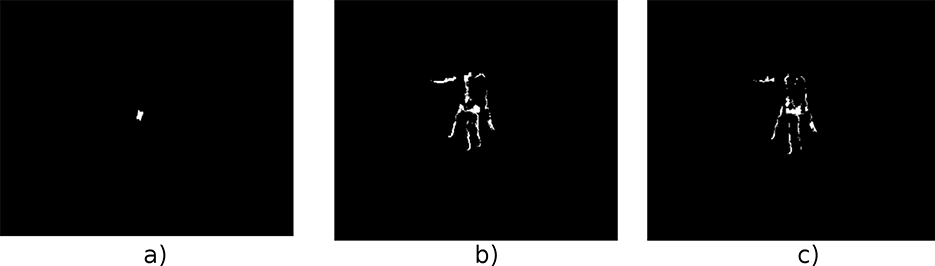
\includegraphics[width=\columnwidth]{images/color_tracking_probs.png}
\caption{Images showing reflection problems with  orange color thresholding. a) Correct threshold with only the marker being thresholded b-c) Depending on the rotaton of the hand, skin reflecton color falls into tracking threshold.}
\label{img:Color_reflecton_problems} 
\end{figure}
Acrylic paint is available in many color variations, making it possible to stay outide of the skintone color ranges for the marker colors.It showed to have the benefits of being easily to apply to the finger. The finger coating is dry in under a minute after application. Adaption for finger size is automatically included in the application process.  
\\\\The implemented ROI feature speed up the whole system calculations once the colors are found. Before this point, the system scans whole frames to find colors, which takes more time than the much smaller ROI regions.
Empirical evaluations showed, that for the used tracking space, a ROI region size offset of 40 px in x and y directions produces the best results in terms of consistency. Smaller region offsets caused the system to use tracking for faster hand motion, which causes system slow down until the tracking has recovered. Generally, larger ROI's produce more constent tracking results at the cost of higher calculation time.
\begin{figure}[H]
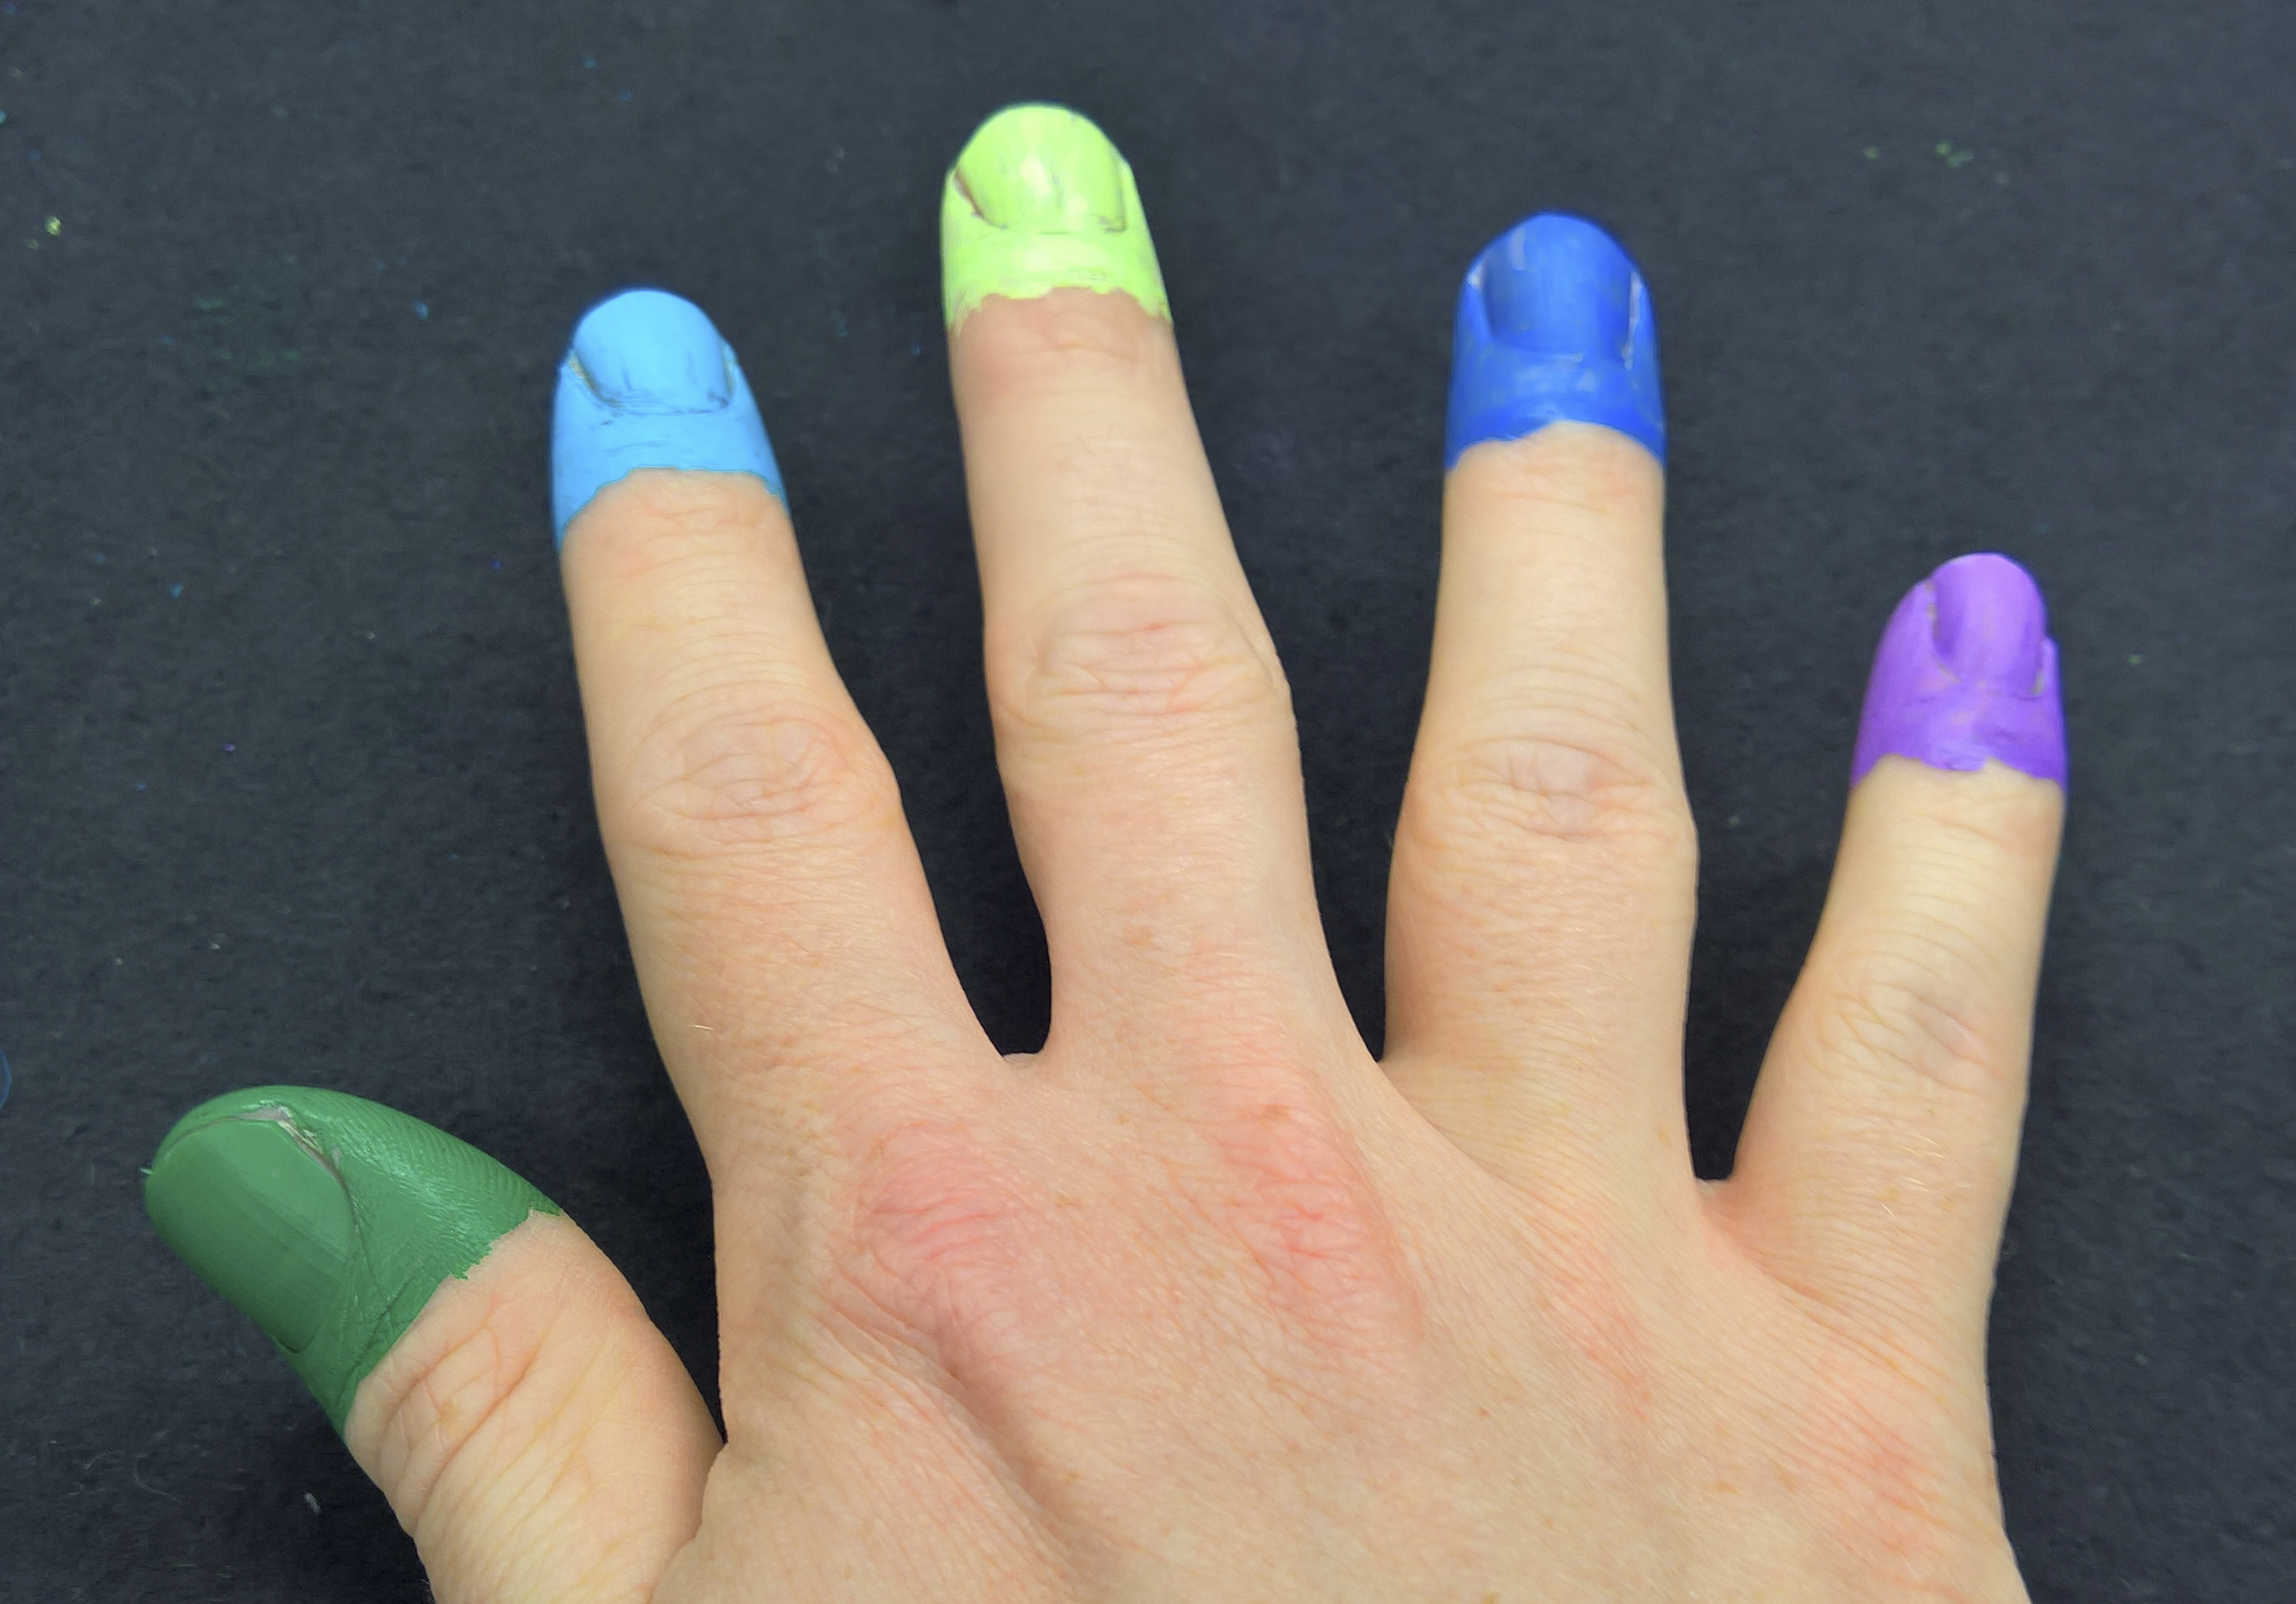
\includegraphics[scale=0.05]{images/final_finger_markers.jpg}
\centering
\caption{Finger marked with suitable acrylic colors}
\label{img:final_markers}
\end{figure}
For the colors a mixture of blue and green color tones together with red tones in the purple and magenta section were chosen as the final colors.
\subsection{Depth measurement accuracy}
To determine the accuracy of the system for it's depth measurement values a simple test bench setup was used. The camera rig was aligned horizontally and fixed to the test bench. A large sized colored marker (75 mm x 50 mm) was used as target for detection. The marker marker was positioned at altering distances from the camera rig along the central axis of the camera rig. The height at which the camera rig is positioned in the experiment setup will be around 100 cm, so the measured distances started at 100 cm from the camera and were decremented in steps of 5 cm until 20 cm in front of the Camera Rig(see Appendix Table \ref{Depth measurement Values} and Figure \ref{char:DisparityToDistanceChart}).
\begin{figure}[H]
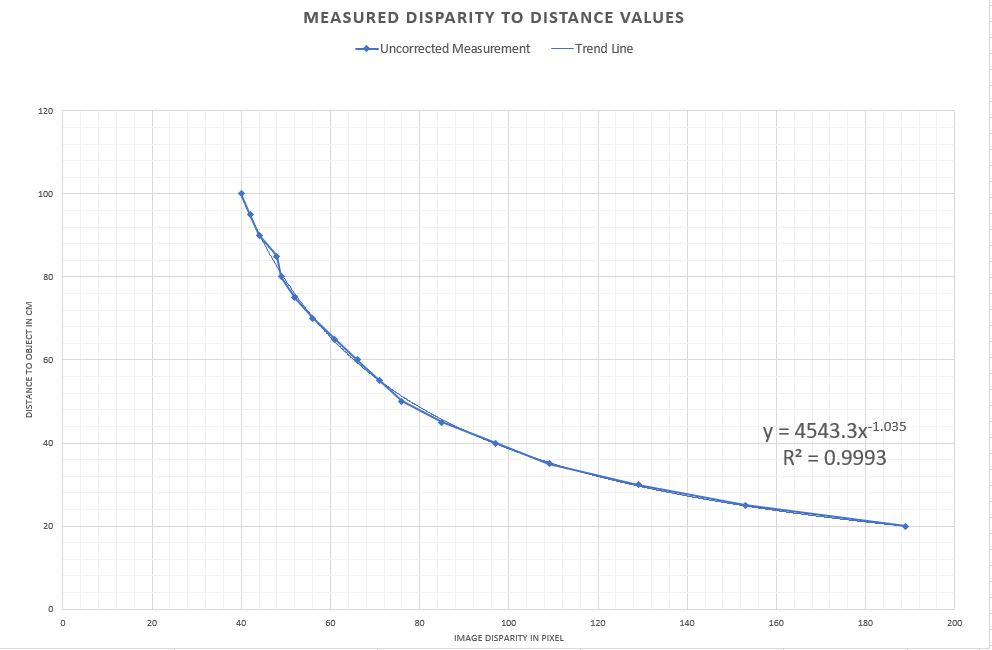
\includegraphics[width=\columnwidth]{images/Disparity_to_distance.JPG}
\caption{Chart showing the results of the disparity measurement with a plotted trend line}
\label{char:DisparityToDistanceChart} 
\end{figure}
The accuracy of the camera system is limited by the number of pixels in relation to the camera view angleas described in \cite{JernejMrovlje.2008}.For the system setup of 640 px image width and a horizontal view angle of $62.5^\circ$, $\Delta\varphi$ is equal to $0.0977\frac{1^\circ}{pixel}$.The system error for a $D=100cm$ would therefore result in about $2cm$ of possible error.As the measured values show deviations of up to $5\%$ from the correct value, the function from the trend line displayed in Figure \ref{char:DisparityToDistanceChart} was taken as a correcting factor for the depth calculation.Values lying on the trend line of Figure \ref{char:DisparityToDistanceChart} should correspond more exactly to the correct distance values \cite{ManafA.Mahammed.2013}, which correspond to the results of :
\begin{equation}
\label{equ:power_function}
D=k*x^{z}
\end{equation}
with K being:
\begin{equation}
k=\frac{Bx_0}{2\tan(\frac{\varphi_0}{2}+\phi)}
\end{equation}
and x the disparity in pixels.
The $\phi$ term in the equation above is used as a compensation for possible alignment errors.
The trend line, which is fit to the measurements in Figure \ref{char:DisparityToDistanceChart} represents the the function needed to fulfill Equation \ref{equ:power_function}.The calculated values are $k=4543.3$ and $z=-1.035$.
With the utilization of the corrected value formula, the accuracy of the depth measurement(see Appendix Table \ref{Depth measurement Values}) are acceptable for the prototype application.
\section{Data filtering}
The finger marker base jitter measurements showed that the systems can only supply a certain stability of position tracking. This results in the fluctuation of the measurement results. When rendering this unfiltered data directly, a large optical jitter in all positions is the case. Jittering of position values also causes the height calculation algorithm to generate incorrect height values.\\
To counter this data jitter, the incoming data-set is filtered in several steps with the \textit{1 euro filter} presented by Casiez et.al. \cite{Casiez.2012}.It uses a first order low-pass filter with an adaptive cutoff frequency to filter noisy signals for high precision and responsiveness. This means that at low speeds, a low cutoff reduces jitter at the expense of lag, but at high speeds, the cutoff is increased to reduce lag rather than jitter.\\
\newpage The filter was chosen, beacuase of a relative simple and easy implementation as well as an uncomplicated setup and tuning process. It also produces faster and better results in comparsion to the normally used \textit{Kalman filter}\cite{Welch.2001}, \textit{moving average filter} or \textit{low-pass filters and exponential smoothing filter}s\cite{LaViola.2003}.
\\ In the first step, the incoming data for each finger and the base marker  are filtered separately and component-wise. This allows for specific fine tuning of the filter values, as each marker shows different jitter. The filtered values are then passed to the depth calculation algorithm where the z position of the respective marker is calculated. The result is also filtered before all components are written into the final result position vector.
\\\\The calibration process of the filter is very simple. The filter needs three base values to function correctly. The first one is the frequency at which the data values are delivered. This can easily be measured from the timestamp differences of the incoming data packages. The other two values are the minimum cutoff frequency$f_{c_{min}} $ of the low pass filter and the slope of the filter curve $\beta$.
\\The other two values have to be calibrated in a manual process for each marker.In the first step the value of $f_{c_{min}} $ is set to one and $\beta$ is set to zero. The markers are held in a static position or moved very slowly to check for jitter. The value of $f_{c_{min}} $ is then adapted to a point where the jitter is minimized without creating to much lag for these slow movements. In the second step, the tracker are moved fast and the $\beta$ value is increased until lag for fast movements is minimized.
\todo{measure filter values}
\section{Inverse kinematics algorithm}
Figure \ref{img:hand-constraint_debug_view} shows the a debugging representation of the used kinematic structure of the \textit{Caliko} framwork. The non-black colored lines of the left picture show the kinematic chains for each finger. The black colored lines are used as an offset structure from the hand base marker.
The kinematic chains all have their own target point for which the algorithm can solve for. All chains are grouped into a kinematic model for easier data handling. The kinematic model provides a container for easier access of the base and the connection structure through which the fingers are connected to the base.
With this data, the algorithm is capable of calculating a solution for each kinematic finger chain and applying these values to the position. If the target is reachable, the digital finger position should match the pose of its real world counterpart up to a specified threshold value.
\begin{figure}[H]
\centering
\includegraphics[width=\columnwidth/2]{images/hand_model_combo.png}
\caption{Hand model representatio of the used IK Framework: a) Kinematic chains and base structure, b) hand model with visualized movement constraints}
\label{img:hand-constraint_debug_view} 
\end{figure}
The right image shows the same model with applied constraints to each chains. The framework differentiates between base bone constraints and normal bone constraints. The base-bone constraints are treated separately as the base-bone is the starting point of the kinematic chain and therefore effects all following bones. In the 3D mode constraints with either a global or a local reference axis can be applied. The local reference axis usually refers to a axis of the previous bone. Global constraints are used for base-bone constraints. The reference Axis can the be used for the specific type of constraint. The framework supports hinge type constraints and rotor constraints. The hinge types define a rotation axis around which the bone can rotate (1 DOF). The rotor-based constraint defines an angle for a cone on a defined axis which limits the movement of the joint in multiple directions (2 DOF). This circular curve limitation  is a downside of the framework as a parabolic curve description for a rotor-based constraint would better fit the movement capabilities of the fingers.
\todo{measure calculation times} 